\documentclass[11pt,a4paper]{article}
\usepackage[T1]{fontenc}\usepackage[utf8]{inputenc}\usepackage[brazil]{babel}
\usepackage{lmodern,microtype,amsmath,booktabs,array,graphicx,float,caption,xcolor,enumitem,fancyhdr,hyperref}
\usepackage[margin=1.9cm,top=1.9cm,bottom=1.9cm]{geometry}
\definecolor{navy}{HTML}{164E63}\hypersetup{colorlinks=true,linkcolor=navy,urlcolor=navy,pdftitle={Prever menos, decidir melhor},pdfauthor={Macroeconomia Aplicada}}
\setlength{\parindent}{0pt}\setlength{\parskip}{6pt}\setlength{\emergencystretch}{3em}
\setlength{\tabcolsep}{5pt}\renewcommand{\arraystretch}{1.1}\setlength{\intextsep}{6pt}\setlength{\textfloatsep}{8pt}
\captionsetup{font=small,labelfont={bf,color=navy},skip=4pt}\setlist{nosep}
\pagestyle{fancy}\fancyhf{}\setlength{\headheight}{15pt}\fancyhead[L]{\small\color{navy}Prever menos, decidir melhor}\fancyhead[R]{\small Síntese econômica | Câmbio e carrego}\fancyfoot[C]{\thepage}
\begin{document}
\thispagestyle{empty}
{\large\color{navy}MACROECONOMIA APLICADA \quad | \quad SÍNTESE FINAL}
\vspace{1.3cm}

{\Huge\bfseries\color{navy}Prever menos,\\[6pt]decidir melhor}
\vspace{.6cm}

{\Large Câmbio real, condições comerciais\\e gestão econômica do carrego}
\vspace{.8cm}

\textbf{Pergunta de pesquisa.} A informação macroeconômica gera mais valor ao escolher a moeda, dimensionar a posição ou decidir quando permanecer exposto?

\textbf{Resultado central.} Uma combinação simples de três módulos preserva aproximadamente o retorno do carry, com menor risco histórico. A maior contribuição está na decisão de exposição e permanência; acrescentar complexidade à previsão não garante valor econômico.
\vspace{.5cm}
\small\begin{center}\begin{tabular}{lrr}\toprule Abr/2018--ago/2026 & Carry puro & Média dos módulos\\\midrule 
Retorno composto anual & 5,78\% & 5,94\%\\
Volatilidade anual & 4,11\% & 2,33\%\\
Maior queda desde o pico & -9,09\% & -1,43\%\\
Sharpe & 0,75 & 1,37\\\bottomrule\end{tabular}\end{center}\normalsize

\vspace{.5cm}
\textbf{Natureza da evidência.} Pesquisa empírica preditiva e avaliação de decisões, com dados e custos explícitos. Não identifica choques causais nem demonstra arbitragem. As combinações são novas, mas a história já foi examinada nos estudos anteriores. A vantagem de retorno não é significativa após controlar a busca na grade principal.

\vfill
Dados congelados até agosto de 2026.\\
Relatório, código, resultados completos e documentação reproduzível.\\
Baseado na aula 8 e em Eichenbaum, Johannsen e Rebelo (2021).

\clearpage
\section*{1. As descobertas que merecem permanecer}

\textbf{A informação pode valer mais na decisão do que no ranking.} Trocar o ranking de juros por juros mais previsão EJR não foi uma boa escolha na amostra. Usar a previsão para dimensionar ou condicionar exposição foi mais útil. Não é a mesma hipótese estatística ou econômica.

\textbf{A carteira melhor não é a interseção de todos os filtros.} Exigir aprovação simultânea de valorização, preços, composição e risco elimina oportunidades. Uma média com pesos iguais permite que os módulos tenham funções e horizontes diferentes.

\textbf{O melhor aprendizado comercial é a adaptação.} Mudanças observadas na composição ajudam mais que tentar prever toda a transformação comercial. A extensão de commodities que melhora alguns erros de cinco anos não melhora automaticamente a carteira líquida.

\textbf{A fonte do prêmio muda.} Na combinação, a contribuição anual de juros cai de 2,62 para 1,50 pontos percentuais em relação ao carry; a contribuição cambial sobe de 0,74 para 1,82. O ganho vem da exposição escolhida, não de receber mais juros.

\textbf{O custo da proteção aparece nos meses bons perdidos.} A combinação fica quase fora do mercado em 2019 e perde uma alta favorável do carry. Em 2020--2021, evita parte relevante da deterioração. Desde 2023, rende menos que carry na média, com menos volatilidade.

\textbf{O resultado não é universal.} BRL e JPY concentram aproximadamente 86\% da contribuição antes dos custos de transação da combinação. Excluir BRL reduz fortemente o ganho econômico absoluto. Não podemos extrapolar a regra para qualquer conjunto de países.

\textbf{No hedge, o ativo continua importando.} BIL e SPY têm riscos próprios diferentes. A mesma operação cambial adiciona praticamente o mesmo retorno aritmético aos dois, mas muda patrimônio, volatilidade e drawdown de formas distintas.

Este relatório prioriza essas descobertas e mostra também as tentativas que falharam. Os arquivos completos mantêm todas as especificações executadas, sem substituir a grade pela sua melhor linha.

\clearpage
\section*{2. Teoria mínima: previsão não é retorno}

Se $S$ é moeda local por USD, uma posição comprada na moeda local ganha com queda de $S$. O retorno de um depósito estrangeiro, convertido em USD, é
\[
R^i_{t+1}=(1+i^i_t)\frac{S_t}{S_{t+1}}-1.
\]
Seu excesso sobre o funding USD contém juros, variação cambial e a interação entre ambos. Com posições compradas e vendidas, remuneração do caixa e custos:
\[
R^p_{t+1}=r^{USD}_t+\sum_i w_{i,t}(R^i_{t+1}-r^{USD}_t)-c_t-b_t.
\]
Não é uma operação de ``só câmbio''. O ativo subjacente do painel é um depósito/passivo curto aproximado por taxas oficiais. A simulação não usa retorno total de títulos longos nem contratos negociáveis observados.

O EJR relaciona o câmbio real atual à variação nominal futura em países com metas de inflação. O argumento econômico é que o ajuste real pode aparecer mais no nominal que na inflação relativa. Nosso projeto replica a relação preditiva e avalia decisões; não replica todo o DSGE identificado do artigo.

Uma previsão de cinco anos é convertida em sinal mensal dividindo a variação log prevista por 60. Isso é uma aproximação de velocidade média, não uma previsão identificada do caminho mensal. Daí a importância de testar tamanho, permanência e perdas no caminho.

A literatura de carry associa o prêmio cambial a riscos que podem aparecer de forma assimétrica. Nosso backtest não mede todos os riscos de liquidez, margem ou execução. Um Sharpe alto sem um episódio extremo na janela não prova que esses riscos desapareceram.

\textbf{Três critérios separados.} Erro de previsão mede acurácia; retorno líquido mede resultado financeiro; certeza equivalente mede uma troca entre média e risco para uma preferência especificada. Uma regra pode melhorar um e piorar outro.

\clearpage
\section*{3. Dados, amostra e o que está identificado}

Reutilizamos o snapshot dos quatro estudos: BRL, EUR, JPY, GBP, CAD e SEK; câmbio mensal de fechamento, CPI, juros e preços comerciais. A amostra de estimação começa em outubro de 1999 e termina em agosto de 2026. A avaliação longa de módulos disponíveis começa em março de 2013. A comparação integral dos módulos começa em abril de 2018, com 101 retornos mensais.

CPI entra com dois meses de atraso e preenchimento de no máximo um mês passado. Commodities usam defasagem de publicação; a extensão específica do terceiro estudo usa preços reais conhecidos com dois meses. Pesos comerciais anuais usam média de três anos, somente até $Y-2$. Alemanha aproxima o comércio da área do euro. Os arquivos atuais contêm revisões e não reconstruem todos os vintages.

\textbf{Identificação.} Este é um exercício de previsão e comparação de políticas condicionais. A variação vem do câmbio real, diferenciais de juros, preços comerciais e sua composição, observados no tempo e entre moedas. Não há instrumento ou experimento que torne essas mudanças exógenas. Portanto, não identificamos o efeito causal dos termos de troca sobre o câmbio, nem o efeito de adotar metas de inflação. Essa limitação responde explicitamente à orientação do professor sobre o que a estratégia empírica identifica.

As previsões são recursivas: cada estimação só admite rótulos realizados e disponíveis antes da origem. Os modelos de risco com informação adicional têm bases reestimadas nas mesmas linhas de treino. O relatório original e seus resultados desfavoráveis continuam preservados.

\textbf{Ponto de partida empírico.} A replicação brasileira dos slides recuperou inclinação de oito anos de -1,808 e $R^2$ de 0,883 na amostra. No painel, o EJR em cinco anos teve RMSE relativo ao passeio aleatório de 1,037. A diferença entre ajuste histórico forte e desempenho preditivo limitado motivou a análise econômica das regras, em vez de presumir lucro a partir do $R^2$.

\textbf{Seleção histórica.} Os componentes foram escolhidos por aprendizado nos estudos anteriores. Não existe uma amostra historicamente intocada nesta entrega. Fixamos combinações simples antes de rodá-las, avaliamos seleção usando só o passado e corrigimos a busca na grade principal. Isso reduz interpretações exageradas, mas não elimina a seleção acumulada em todo o projeto.

\clearpage
\section*{4. Uma política com três funções econômicas}

O ponto de partida é o carry: duas pernas compradas e duas vendidas, 25\% cada, escolhidas pelo diferencial de juros. A conta tem colateral em USD; a exposição bruta máxima é um. A síntese combina três módulos:

\textbf{A. Dimensionar e adaptar.} O sinal agregado soma o diferencial mensal de juros à apreciação EJR prevista, dividida pelo horizonte. O tamanho é o sinal atual dividido por sua mediana histórica anterior, limitado a $[0,1]$. Um alerta de mudança observada da composição comercial retira o par afetado. O limite é o percentil 80 passado da soma das mudanças absolutas dos pesos em três anos.

\textbf{B. Exigir remuneração e evitar deterioração.} O carry só é aberto quando seu retorno previsto agregado, suavizado por seis meses, supera 2\% a.a. Pares são retirados quando o índice comercial em 12 meses deteriora para a perna comprada ou melhora contra a perna vendida, acima do percentil de risco histórico.

\textbf{C. Controlar a permanência.} Coortes mensais de pares recebem orçamento $1/12$ e duram até 12 meses. Um aumento positivo da probabilidade de o câmbio consumir o carry, além do percentil 80 passado, impede entrada ou fecha a coorte. A direção do alerta acompanha a posição aberta, mesmo se o diferencial de juros atual mudar de sinal.

A combinação principal é
\[
w^{\mathrm{média}}_t=\frac13w^A_t+\frac13w^B_t+\frac13w^C_t.
\]
Os pesos são combinados antes de calcular custos e empréstimos. Não há otimização de Sharpe. Posições retiradas ficam em caixa. A versão ``núcleo + média'' mantém 50\% do orçamento no carry e 50\% na combinação.

Essa arquitetura permite discordância: tamanho responde à remuneração, condições comerciais à fragilidade e coortes à permanência. A alternativa de multiplicar todos os filtros também é testada, em vez de presumir que mais restrições são melhores.

\clearpage
\section*{5. Comparação principal em datas iguais}
\footnotesize\begin{center}\begin{tabular}{lrrrrr}\toprule Regra & CAGR & Excesso & Vol. & Sharpe & Queda\\\midrule 
Carry puro & 5,78\% & 3,07\% & 4,11\% & 0,75 & -9,09\%\\
Ranking EJR & 2,51\% & -0,09\% & 3,77\% & -0,03 & -7,01\%\\
Tamanho EJR & 5,92\% & 3,20\% & 4,03\% & 0,80 & -8,83\%\\
Filtro EJR & 5,86\% & 3,09\% & 2,42\% & 1,31 & -2,15\%\\
Tamanho + composição & 6,13\% & 3,36\% & 2,88\% & 1,17 & -3,37\%\\
Filtro + preços & 5,38\% & 2,62\% & 2,08\% & 1,25 & -0,72\%\\
Coortes sem saída & 5,49\% & 2,78\% & 3,80\% & 0,74 & -9,92\%\\
Coortes + risco & 6,30\% & 3,51\% & 2,74\% & 1,29 & -1,72\%\\
Coortes integradas & 5,75\% & 2,98\% & 2,47\% & 1,21 & -1,65\%\\
Todos os filtros & 5,33\% & 2,59\% & 2,46\% & 1,04 & -3,37\%\\
Previsão comercial 50\% & 5,90\% & 3,18\% & 3,96\% & 0,81 & -8,44\%\\
Média de dois módulos & 5,76\% & 2,99\% & 2,20\% & 1,36 & -1,41\%\\
Média de três módulos & 5,94\% & 3,17\% & 2,33\% & 1,37 & -1,43\%\\
Núcleo carry + média & 5,87\% & 3,12\% & 3,04\% & 1,04 & -4,71\%\\\bottomrule\end{tabular}\end{center}\normalsize

Abril de 2018 a agosto de 2026. CAGR é crescimento composto líquido em USD; excesso é média aritmética anualizada sobre caixa USD; volatilidade usa retornos totais e Sharpe usa excessos. Queda é o drawdown máximo, com caixa e custos incluídos.

\textbf{Resultado de síntese.} A média de três módulos tem retorno composto de 5,94\% a.a., versus 5,78\% do carry. Sua volatilidade é 2,33\%, versus 4,11\%, e o Sharpe sobe de 0,75 para 1,37. A maior queda observada passa de 9,09\% para 1,43\%.

O módulo de coortes por risco tem maior retorno e certeza equivalente nesta janela, mas a média é a síntese principal por construção econômica e ausência de pesos otimizados. A regra que exige todos os filtros entrega menos retorno que a média, sem melhor drawdown.

Não se deve comparar estes números diretamente com os retornos desde 2010 do primeiro estudo ou chamar a diferença de alfa: as datas e o desenho mudaram. Todas as comparações desta tabela compartilham o calendário.

\clearpage
\section*{6. A trajetória importa mais que o número final}
\begin{figure}[H]\centering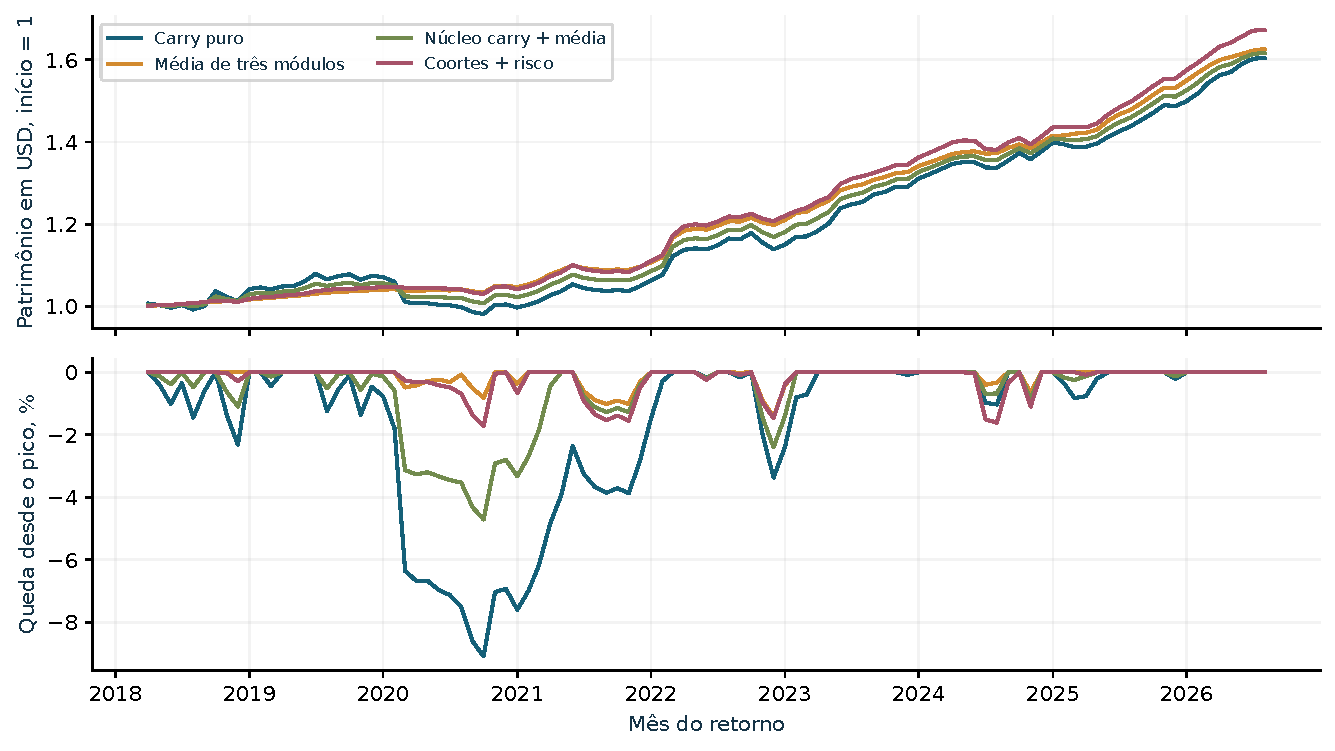
\includegraphics[width=.98\linewidth]{figures/wealth.pdf}\caption{Comparação líquida em USD. A média reduz quedas, mas também fica para trás em alguns meses favoráveis ao carry.}\end{figure}
A trajetória mostra por que a política pode ter valor para um orçamento de risco limitado: o investidor atravessa perdas menores para obter patrimônio final parecido. O módulo de coortes por risco e a média evitam boa parte do caminho negativo concentrado em 2020--2021.

Essa proteção é histórica e condicional à janela. A média ainda perdeu dinheiro em meses individuais; sua pior perda mensal foi -0,90\%. A perda média nos piores 5\% dos meses foi -0,60\%. Não estamos estimando um limite máximo de perda futura.

O teste não inclui a crise financeira de 2008 na avaliação dessas regras, porque os sinais recursivos completos ainda não existiam. A ausência desse episódio é uma limitação relevante para qualquer interpretação de risco de carry.

\clearpage
\section*{7. A contribuição marginal de cada ideia}
\begin{figure}[H]\centering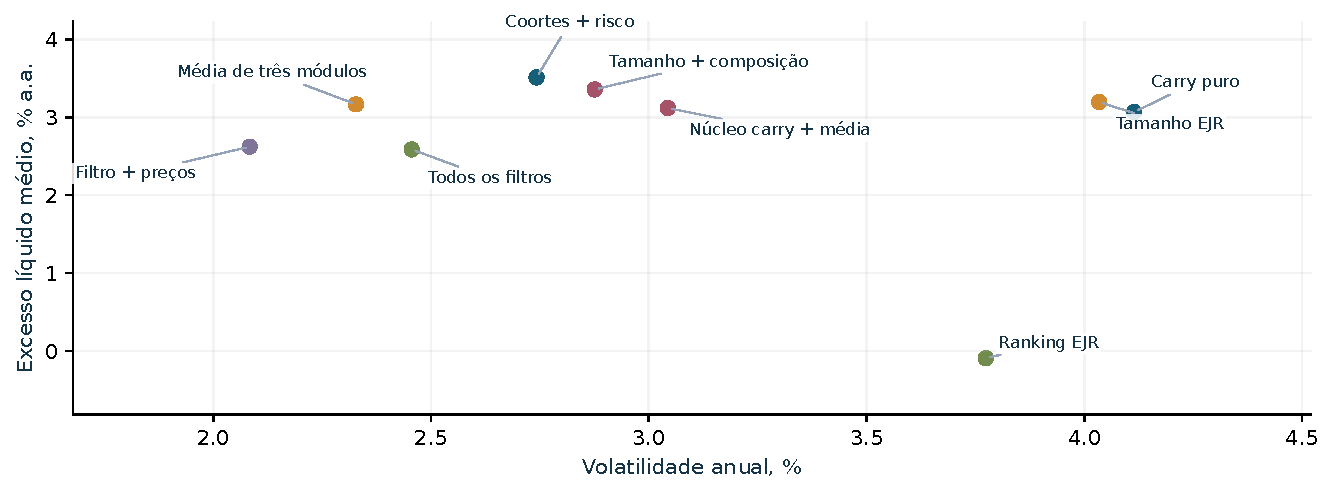
\includegraphics[width=.98\linewidth]{figures/risk_return.pdf}\caption{Mais filtros não deslocam automaticamente a relação entre retorno e risco para uma posição melhor.}\end{figure}\small\begin{center}\begin{tabular}{lrr}\toprule Comparação & $\Delta$ excesso, p.p. a.a. & $\Delta$ CE, p.p. a.a.\\\midrule 
Tamanho EJR / carry & 0,13 & 0,15\\
Composição / tamanho & 0,16 & 0,35\\
Preços / filtro EJR & -0,47 & -0,44\\
Saída / coortes & 0,73 & 0,90\\
Terceiro módulo / média de dois & 0,18 & 0,16\\
Interseção / média & -0,58 & -0,60\\\bottomrule\end{tabular}\end{center}\normalsize

A contribuição depende da função. Preços sobre o filtro EJR reduzem retorno, mas produzem uma trajetória de menor risco. A saída das coortes melhora ambos nesta janela. Acrescentar o terceiro módulo à média aumenta ligeiramente retorno e certeza equivalente, mas a média de dois já captura boa parte da melhora de Sharpe.

Estas diferenças são remoções/substituições de módulos, não efeitos causais independentes. Os sinais têm correlação, regras de entrada diferentes e frequências distintas. Uma decomposição de retorno não identifica o mecanismo estrutural que gerou cada ganho.

\clearpage
\section*{8. De onde vem o dinheiro?}
\begin{figure}[H]\centering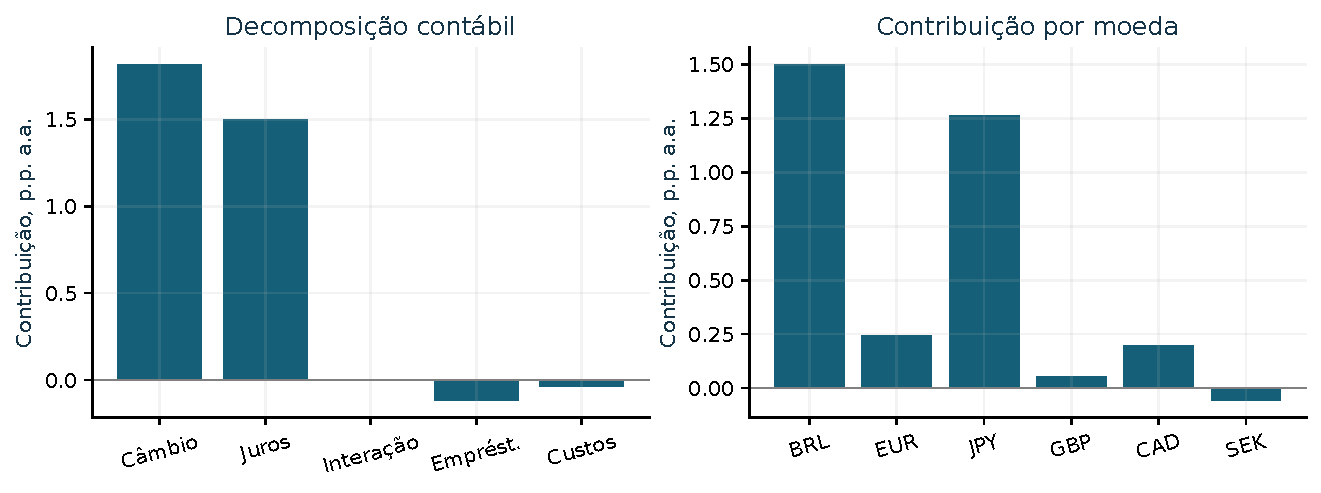
\includegraphics[width=.98\linewidth]{figures/attribution.pdf}\caption{Contribuições aritméticas da média de módulos. A soma das moedas exclui apenas o custo de transação; a soma dos cinco componentes reconcilia exatamente o excesso líquido.}\end{figure}\small\begin{center}\begin{tabular}{lrr}\toprule Componente & Carry, p.p. a.a. & Média, p.p. a.a.\\\midrule 
Câmbio & 0,741 & 1,816\\
Juros líquidos de funding & 2,619 & 1,501\\
Interação juros/câmbio & -0,002 & 0,004\\
Spread de empréstimo & -0,249 & -0,120\\
Transações & -0,040 & -0,036\\\bottomrule\end{tabular}\end{center}\normalsize

O carry puro recebe mais juros; a média obtém maior contribuição cambial com menos exposição. Isso é compatível com a hipótese original de usar informação macro para escolher quando suportar o risco cambial do carrego. Mas a decomposição é contábil: não prova que o sinal previu causalmente uma mudança de regime.

A compensação de ordens entre módulos economiza aproximadamente 0,25 ponto-base por ano nesta amostra. Logo, a melhora não é explicada por um grande benefício oculto de compensação contábil. O efeito vem principalmente das posições e dos momentos em que são mantidas.

\clearpage
\section*{9. Quanto da proteção é simplesmente menor exposição?}
\begin{figure}[H]\centering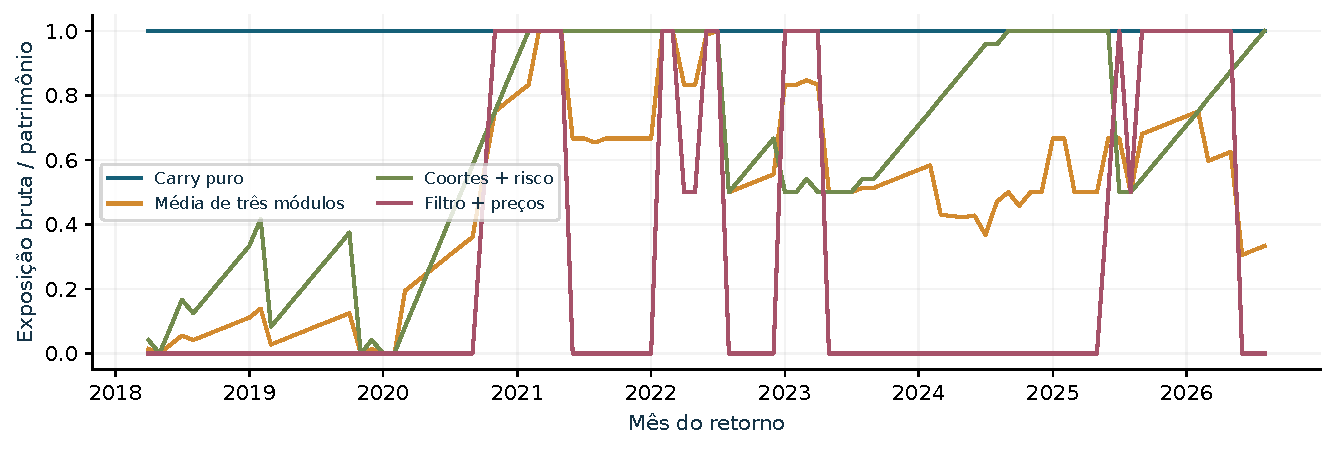
\includegraphics[width=.98\linewidth]{figures/exposure.pdf}\caption{A exposição média da combinação é cerca de 48\% do patrimônio. Ficar em caixa é parte deliberada da política.}\end{figure}\small\begin{center}\begin{tabular}{lrrrr}\toprule Regra & Exp. & Excesso & Vol. & Queda\\\midrule 
Carry & 100,00\% & 3,07\% & 4,11\% & -9,09\%\\
Média dos módulos & 48,03\% & 3,17\% & 2,33\% & -1,43\%\\
Carry / média ex post & 48,03\% & 1,47\% & 2,04\% & -4,02\%\\
Carry / exposição passada & 29,36\% & 1,34\% & 1,30\% & -1,05\%\\\bottomrule\end{tabular}\end{center}\normalsize

O controle ex post iguala a exposição média, mas usa a média futura e serve apenas como diagnóstico. O controle passado usa informações disponíveis, porém sua exposição realizada difere por causa da adaptação lenta do histórico.

À mesma exposição média, a combinação tem volatilidade um pouco maior, retorno maior e drawdown menor que o carry reduzido. O intervalo da diferença de drawdown contra esse controle inclui zero. Portanto, o resultado sugere seleção útil de retorno; não estabelece proteção superior com o mesmo orçamento de exposição.

\clearpage
\section*{10. Medindo valor econômico, além do Sharpe}

Usamos uma aproximação de certeza equivalente excedente para preferências média-variância:
\[
CE_\gamma=12\left(\overline{R-r_f}-\frac\gamma2\,\widehat{\mathrm{Var}}(R-r_f)\right),\quad \gamma\in\{3,5,10\}.
\]
Ela põe retorno e variância na mesma unidade anual. Não é utilidade esperada exata sob caudas assimétricas. O parâmetro representa preferência; não foi escolhido para maximizar a vantagem da estratégia.
\small\begin{center}\begin{tabular}{lrrr}\toprule Regra & CE $\gamma$=3 & CE $\gamma$=5 & CE $\gamma$=10\\\midrule 
Carry puro & 2,82\% & 2,65\% & 2,24\%\\
Filtro EJR & 3,01\% & 2,95\% & 2,81\%\\
Tamanho + composição & 3,23\% & 3,15\% & 2,95\%\\
Coortes + risco & 3,40\% & 3,33\% & 3,14\%\\
Média de dois módulos & 2,92\% & 2,87\% & 2,75\%\\
Média de três módulos & 3,09\% & 3,03\% & 2,90\%\\
Núcleo carry + média & 2,98\% & 2,89\% & 2,67\%\\\bottomrule\end{tabular}\end{center}\normalsize
\begin{figure}[H]\centering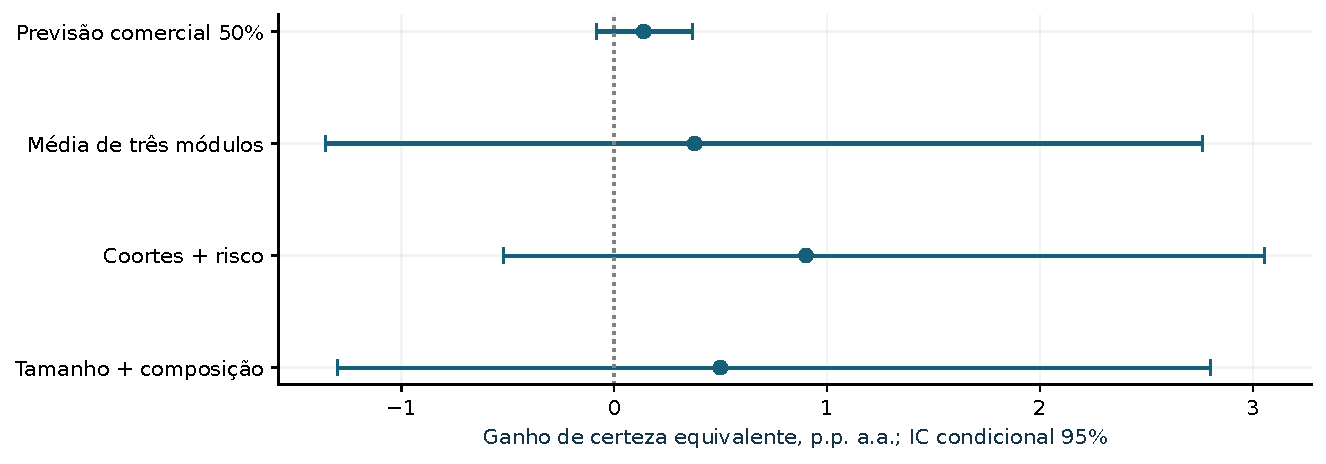
\includegraphics[width=.98\linewidth]{figures/uncertainty.pdf}\caption{Intervalos condicionais em blocos de 12 meses para a diferença contra a base. A vantagem média de utilidade não é estabelecida para a combinação frente ao carry pleno.}\end{figure}
Para $\gamma=5$, a média supera o carry em aproximadamente 38 pontos-base anuais de certeza equivalente. Essa é uma margem econômica amostral antes de uma eventual taxa adicional de gestão; não é uma taxa recomendada nem um ganho garantido. Seu intervalo de 95\% inclui valores negativos.

\clearpage
\section*{11. Quando funciona e quando custa caro}
\begin{figure}[H]\centering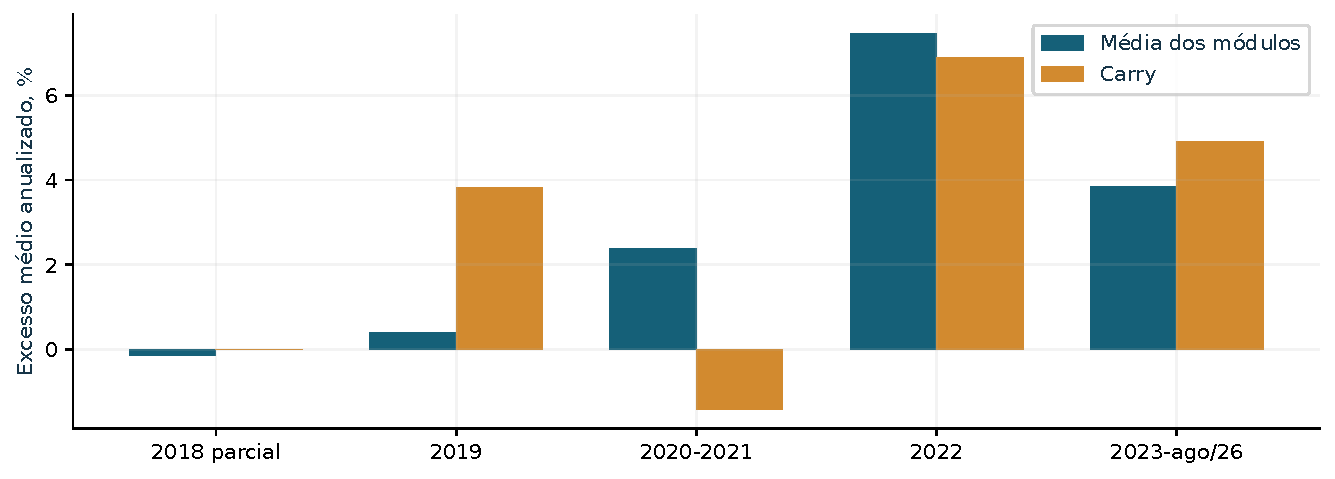
\includegraphics[width=.98\linewidth]{figures/episodes.pdf}\caption{Janelas de calendário fixadas para diagnóstico. Anualizar uma janela curta não cria mais observações nem identifica o efeito causal de um evento.}\end{figure}
\textbf{2019: custo de oportunidade.} A média entrega cerca de 0,40\% a.a. de excesso, enquanto carry entrega 3,83\%. Os módulos de composição e de filtro estão quase sempre em caixa. A proteção pode parecer inútil durante um período favorável.

\textbf{2020--2021: principal contribuição de proteção.} O carry tem excesso médio anualizado de -1,43\%, e a média de módulos, +2,39\%. A menor participação em posições desfavoráveis compensa o custo de ter ficado de fora antes.

\textbf{2022: participação em parte do prêmio.} A média obtém 7,46\% de excesso anual, contra 6,89\% do carry, com menor exposição média. Esse resultado ajuda o desempenho total, mas não deve ser tratado como padrão garantido para todo choque monetário.

\textbf{2023--agosto de 2026: menor retorno com menor risco.} A média entrega 3,85\% a.a. de excesso contra 4,90\% do carry. A estratégia troca parte da alta por uma trajetória menos volátil.

Na pior janela móvel de 36 meses, o excesso anualizado da média foi 0,67\%, contra -0,86\% do carry. A evidência depende de poucos episódios macroeconômicos, apesar das 101 observações mensais.

\clearpage
\section*{12. O Brasil é parte da estratégia, não um detalhe}
\small\begin{center}\begin{tabular}{lrrrr}\toprule Universo & Regra & Excesso & Vol. & CE $\gamma$=5\\\midrule 
Completo & Carry puro & 3,07\% & 4,11\% & 2,65\%\\
Completo & Coortes + risco & 3,51\% & 2,74\% & 3,33\%\\
Completo & Média de três módulos & 3,17\% & 2,33\% & 3,03\%\\
Sem BRL & Carry puro & 2,00\% & 2,78\% & 1,81\%\\
Sem BRL & Coortes + risco & 1,53\% & 1,43\% & 1,48\%\\
Sem BRL & Média de três módulos & 0,65\% & 0,78\% & 0,64\%\\
Sem EUR & Carry puro & 2,77\% & 4,25\% & 2,33\%\\
Sem EUR & Coortes + risco & 3,58\% & 2,90\% & 3,38\%\\
Sem EUR & Média de três módulos & 2,50\% & 2,01\% & 2,40\%\\\bottomrule\end{tabular}\end{center}\normalsize

Retirar BRL derruba o excesso da média de 3,17\% para 0,65\% a.a. A volatilidade cai junto. O Sharpe ainda fica perto de um, mas a certeza equivalente fica muito abaixo do carry do universo sem BRL. Um Sharpe razoável com pouca exposição não resolve a falta de retorno econômico absoluto.

As exclusões refazem o ranking e as regras de posição no universo restante. As previsões de risco reaproveitadas continuam estimadas no painel original; esta é uma sensibilidade de alocação, não uma estimação inteiramente sem informação brasileira.

Parte do mecanismo é a barreira absoluta de 2\% a.a.: com prêmios menores, um módulo quase desliga. Investigamos depois da primeira rodada barreiras de zero e metade da mediana histórica do prêmio. Sem BRL, a média sobe de 0,65\% para aproximadamente 0,87\% a.a., ainda abaixo do carry de 2,00\%.

\textbf{Aprendizado de mercado.} O nível mínimo de remuneração aceitável depende do universo, dos custos e do mandato. Um parâmetro plausível para seis moedas não pode ser transplantado sem avaliar como altera a participação. Esse diagnóstico ajuda a entender a regra; não autoriza escolher retrospectivamente uma barreira que restaure o melhor backtest.

\clearpage
\section*{13. Custos, atraso, orçamento de risco e parâmetros}
\begin{figure}[H]\centering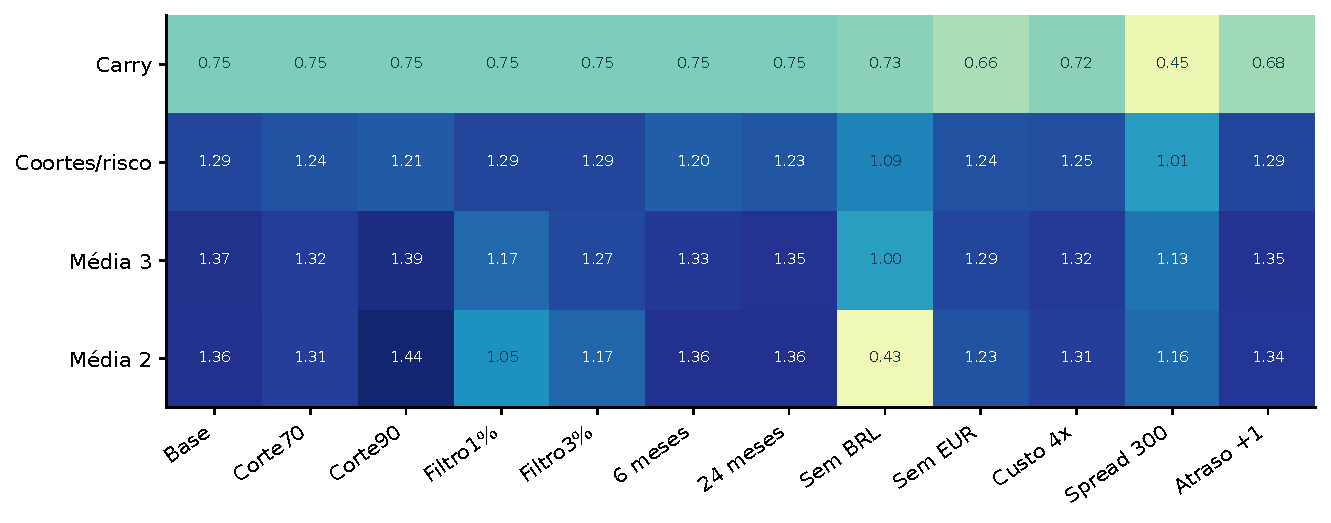
\includegraphics[width=.98\linewidth]{figures/robustness.pdf}\caption{Sharpe nas variantes. O desenho principal é a coluna Base; as demais são sensibilidades e não candidatos escolhidos pela maior célula.}\end{figure}\small\begin{center}\begin{tabular}{lrrr}\toprule Condição & Carry: excesso & Média: excesso & Média: queda\\\midrule 
Base & 3,07\% & 3,17\% & -1,43\%\\
Transações 4 vezes & 2,95\% & 3,06\% & -1,43\%\\
Empréstimo 300 pb/ano & 1,82\% & 2,57\% & -1,55\%\\
Execução mais um mês & 2,76\% & 3,22\% & -1,35\%\\
Redução para alvo 3\% & 2,39\% & 2,57\% & -1,43\%\\\bottomrule\end{tabular}\end{center}\normalsize

A combinação é relativamente estável aos custos e ao atraso adicional nesta amostra, em parte por negociar menos risco que carry. O spread de empréstimo importa mais que pequenos custos por transação porque incide continuamente sobre a perna vendida.

Alvos de volatilidade 3/4/5\% usam covariância de 24 meses observada antes da execução. Só reduzem posições; não há alavancagem para alcançar a meta. O carry com alvo de 3\% já reduz bastante sua queda, reforçando a necessidade de compará-lo com controles simples.

A tabela completa contém 390 linhas de métricas de sensibilidade, incluindo mudanças que não afetam certos módulos. Contá-las como 390 descobertas independentes seria incorreto.

\clearpage
\section*{14. Escolher o vencedor recente foi pior que combinar}
\begin{figure}[H]\centering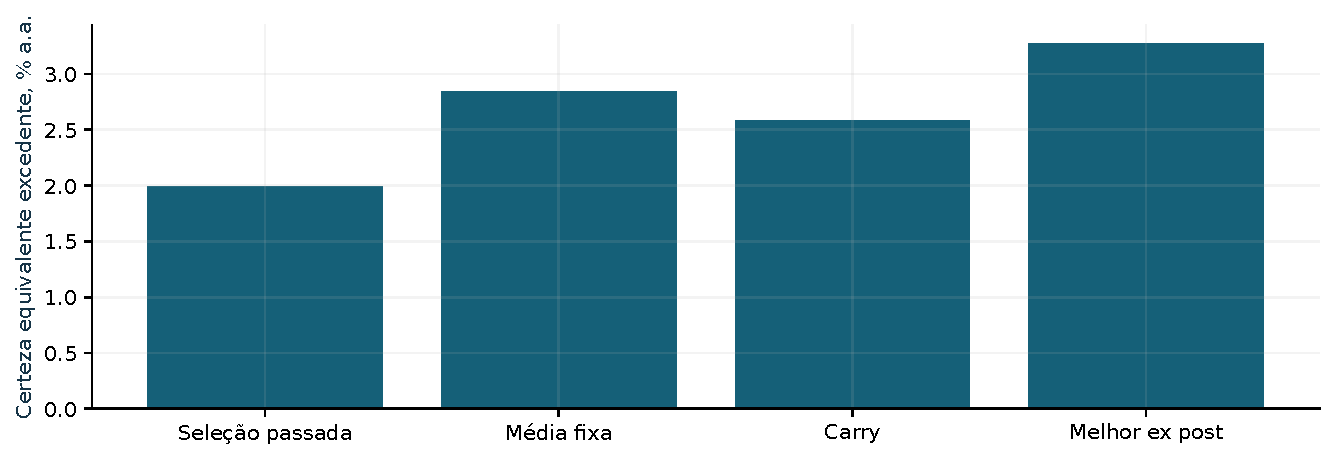
\includegraphics[width=.98\linewidth]{figures/selection.pdf}\caption{Família longa, escolha anual com janela de 36 meses. A seleção ex post é apenas um teto ilustrativo: usa o resultado futuro para identificar o membro vencedor.}\end{figure}\footnotesize\begin{center}\begin{tabular}{lrrrr}\toprule História & Regra & Início & Sharpe & CE $\gamma$=5\\\midrule 
36 & Escolha passada & 2016-05 & 0,78 & 1,99\%\\
36 & Média fixa & 2016-05 & 1,06 & 2,84\%\\
36 & Carry & 2016-05 & 0,74 & 2,59\%\\
36 & Melhor ex post & 2016-05 & 1,17 & 3,28\%\\
60 & Escolha passada & 2018-05 & 0,65 & 1,75\%\\
60 & Média fixa & 2018-05 & 1,07 & 2,88\%\\
60 & Carry & 2018-05 & 0,74 & 2,61\%\\
60 & Melhor ex post & 2018-05 & 1,18 & 3,18\%\\\bottomrule\end{tabular}\end{center}\normalsize

Todo janeiro, a regra escolhe o membro com maior certeza equivalente nos últimos 36 ou 60 meses, usando apenas retornos até o mês anterior. Mantém essa escolha até a próxima atualização, com execução atrasada e custos da carteira resultante.

Nas duas janelas da família longa, a escolha passada perde para a média fixa. A família com todos os sinais começa a ser selecionável mais tarde e também não mostra vantagem consistente de perseguir o melhor desempenho recente.

Isso não prova que toda adaptação é ruim. Mostra que o erro de escolher qual regra dominará o próximo regime pode superar o benefício da flexibilidade. Com amostra curta e sinais persistentes, pesos iguais são uma disciplina econômica útil, além de uma simplificação operacional.

\clearpage
\section*{15. Uma previsão melhor pode dar uma carteira pior}

O terceiro estudo encontrou melhora de erro nominal em cinco anos ao incluir um componente de commodities específico à composição comercial. Reproduzimos essa previsão e combinamos 50\% dela com 50\% do EJR. A carteira usa o resultado combinado para dimensionar carry. Também variamos esse peso para 25/75\%.
\small\begin{center}\begin{tabular}{lrrrr}\toprule Janela & Sinal & Excesso & Sharpe & CE $\gamma$=5\\\midrule 
Desde 2013 & Tamanho EJR & 2,81\% & 0,69 & 2,40\%\\
Desde 2013 & Previsão comercial 50\% & 2,28\% & 0,58 & 1,90\%\\
Desde 2018 & Tamanho EJR & 3,20\% & 0,80 & 2,80\%\\
Desde 2018 & Previsão comercial 50\% & 3,18\% & 0,81 & 2,79\%\\\bottomrule\end{tabular}\end{center}\normalsize

Na janela longa, o blend comercial tem excesso de 2,28\% a.a., contra 2,81\% do tamanho EJR. Na janela comum, os resultados são muito próximos. A melhora estatística de um endpoint distante não se traduz em uma trajetória mensal mais remuneradora depois de juros e custos.

\textbf{Uma tentativa economicamente mais direta também falhou.} Estimamos a probabilidade de perda de 15 pares, incluindo sua volatilidade e informação comercial conjunta. Avaliamos só os dois pares efetivamente escolhidos a cada origem. O Brier relativo é 1,011, com 90 datas avaliadas: não melhora a base.
\small\begin{center}\begin{tabular}{lrrr}\toprule Regra de permanência & Excesso & Sharpe & Queda\\\midrule 
Risco conjunto do par & 0,51\% & 0,18 & -9,92\%\\
Risco orientado das pernas & 3,51\% & 1,29 & -1,72\%\\
Coortes sem saída & 2,78\% & 0,74 & -9,92\%\\
Média com risco do par & 2,17\% & 1,02 & -3,31\%\\\bottomrule\end{tabular}\end{center}\normalsize

Esse resultado negativo impede que a síntese se torne apenas uma coleção de acertos. Uma hipótese economicamente plausível pode falhar por pouco sinal, excesso de parâmetros ou instabilidade; sua plausibilidade não substitui validação.

\clearpage
\section*{16. Permanência: o desenho correto da posição}

Uma coorte guarda quais moedas foram compradas e vendidas na entrada. A regra de saída deve avaliar o risco \emph{dessa posição}; não pode simplesmente usar a direção favorecida pelo diferencial de juros atual.

No modelo de risco herdado, o evento é o câmbio consumir o diferencial de juros em 12 meses, orientado pela posição de carry em cada origem. Para a síntese, convertemos a mudança de probabilidade para a perna comprada ou vendida efetivamente mantida. Para direção oposta, usamos o complemento do evento log de perda, uma aproximação que não inclui custos nesse rótulo preditivo. A contabilidade da carteira inclui os custos.

Também exigimos aumento positivo do risco, além do percentil histórico. Uma variação apenas menos negativa não basta. Por essas razões, este módulo é uma \textbf{nova especificação}, e seu drawdown de 1,72\% não deve ser apresentado como reprodução dos 3,23\% encontrados no complemento anterior.

Coortes são fechadas no primeiro sinal admissível ou no vencimento. A informação em $t$ produz operação em $t+1$ e retorno em $t+2$. Encerrar a coorte retira o risco; não transfere o orçamento retirado para multiplicar a exposição de outra coorte. Novas entradas mensais são decisões distintas.

A base de comparação abre coortes nas mesmas datas, com a mesma formação gradual. Isso evita atribuir ao filtro o simples benefício de começar com menos capital alocado.

O resultado econômico é atraente nesta janela: excesso de 3,51\% a.a. contra 2,78\% da base, com menor drawdown. Seu ganho de certeza equivalente frente à base tem intervalo amplo que inclui zero. Permanece um candidato de pesquisa, não uma política de saída comprovada.

\clearpage
\section*{17. Mercado: a mesma previsão aplicada ao hedge}
\begin{figure}[H]\centering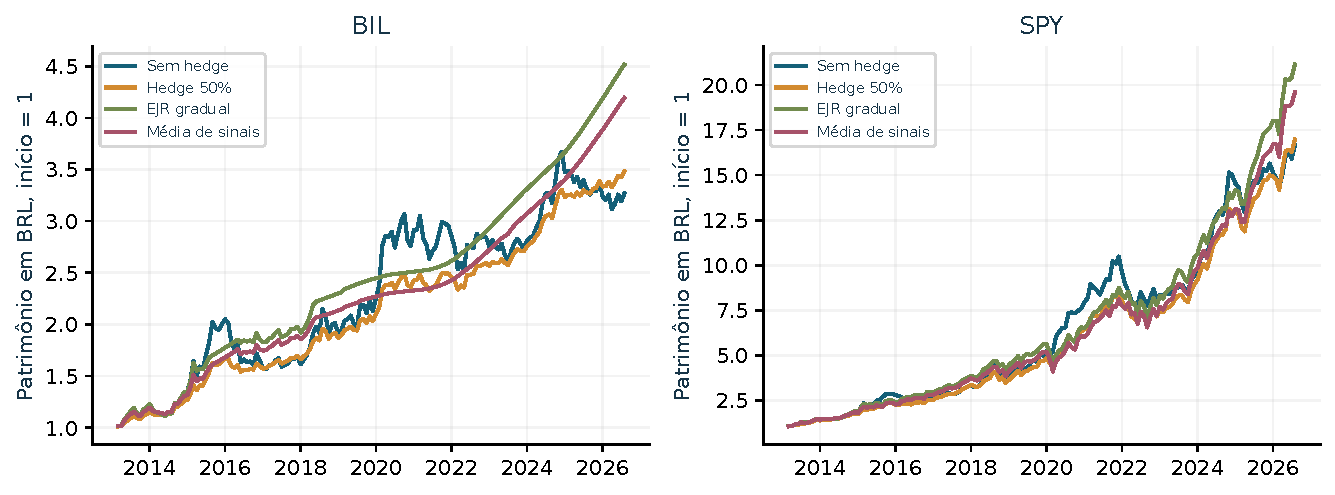
\includegraphics[width=.98\linewidth]{figures/hedge_wealth.pdf}\caption{Ativos americanos mantidos continuamente, com resultados em BRL desde março de 2013. O painel do SPY usa escala própria por seu prêmio acionário.}\end{figure}
Aqui a pergunta muda: um investidor em BRL já possui BIL ou SPY e escolhe quanto do risco USD/BRL proteger. Ele não vende o ativo para ir a caixa. O retorno do ETF e o overlay cambial são registrados separadamente.

Testamos hedge 0/50/100\%, EJR gradual, retorno total gradual, blend comercial, média das três previsões e metade hedge 50\% mais metade sinal. A média reduz a sensibilidade a uma previsão específica, sem otimizar pesos.

O hedge mensal é aproximado por um forward sintético com diferencial de juros. A execução tem o mesmo atraso; cobramos custo por notional rolado, variando 2/5/10 pontos-base. O ativo recebe custo de entrada e saída. Não possuímos cotações históricas executáveis de forwards ou swaps cambiais, base, margem e limites de contraparte.

As taxas aqui não são diretamente comparáveis às carteiras em USD. O numerário, o ativo e o benchmark de caixa são BRL. Um retorno nominal alto em BRL pode refletir juros locais, inflação, prêmio acionário e câmbio, não a capacidade do modelo.

\clearpage
\section*{18. A escolha do ativo muda o valor do hedge}
\footnotesize\begin{center}\begin{tabular}{lrrrr}\toprule Ativo / hedge & CAGR BRL & Vol. & Queda & Hedge médio\\\midrule 
BIL / zero & 9,17\% & 14,99\% & -23,53\% & 0,00\%\\
BIL / 50\% & 9,69\% & 7,47\% & -7,99\% & 50,00\%\\
BIL / 100\% & 9,60\% & 1,05\% & 0,00\% & 100,00\%\\
BIL / EJR gradual & 11,82\% & 6,73\% & -9,58\% & 72,24\%\\
BIL / média & 11,20\% & 4,96\% & -5,16\% & 78,97\%\\
BIL / 50\% + sinal & 10,49\% & 5,55\% & -4,02\% & 64,48\%\\
SPY / zero & 23,18\% & 17,18\% & -26,34\% & 0,00\%\\
SPY / 50\% & 23,34\% & 13,94\% & -22,61\% & 50,00\%\\
SPY / 100\% & 22,82\% & 14,40\% & -21,24\% & 100,00\%\\
SPY / EJR gradual & 25,36\% & 15,48\% & -21,24\% & 72,24\%\\
SPY / média & 24,66\% & 14,87\% & -21,20\% & 78,97\%\\
SPY / 50\% + sinal & 24,06\% & 14,08\% & -20,87\% & 64,48\%\\\bottomrule\end{tabular}\end{center}\normalsize

\textbf{BIL.} O ativo tem pouco risco próprio de preço em USD. Por isso, a proteção cambial reduz muito a volatilidade em BRL. Hedge integral aproxima o resultado do carry implícito nos juros locais, mas não remove risco de implementação. O EJR gradual teve maior retorno nesta amostra, com mais risco que hedge integral.

\textbf{SPY.} O ativo mantém risco acionário. Mesmo com hedge, o drawdown permanece acima de 20\%. O hedge 50\% reduz volatilidade em relação a zero e 100\% nesta história; a covariância entre ações e dólar importa. Não usamos o câmbio para afirmar que prevemos o prêmio acionário.

A diferença aritmética entre aplicar o mesmo hedge a BIL e SPY é praticamente idêntica: o overlay protege um notional USD inicial. A diferença de CAGR não é idêntica porque a composição no tempo interage com a trajetória do ativo. Esse é um resultado contábil auditado, não dois testes independentes que confirmam alfa.

Os intervalos de ganho do hedge dinâmico contra hedge fixo e média de exposição ex post incluem zero. O valor mais defensável aqui é alinhar risco cambial ao mandato e ao ativo mantido; o timing lucrativo permanece incerto.

\clearpage
\section*{19. Controle da busca e confiança nas descobertas}

Testar muitas regras aumenta a chance de encontrar uma curva atraente por acaso. Reamostramos em blocos de 12 e 36 meses as diferenças de retorno de 14 alternativas frente ao carry, preservando sua dependência conjunta. Centralizamos as diferenças e usamos a maior estatística padronizada em cada réplica para um controle max-t unilateral na grade principal.
\small\begin{center}\begin{tabular}{lrrr}\toprule Regra & $\Delta$ excesso a.a. & p ajustado 12m & p ajustado 36m\\\midrule 
Tamanho EJR & 0,13\% & 0,435 & 0,231\\
Tamanho + composição & 0,29\% & 0,886 & 0,935\\
Coortes + risco & 0,44\% & 0,814 & 0,823\\
Média de três módulos & 0,10\% & 0,929 & 0,975\\
Previsão comercial 50\% & 0,11\% & 0,578 & 0,305\\\bottomrule\end{tabular}\end{center}\normalsize

Nenhuma dessas vantagens médias de retorno é significativa nesse teste. Os p-valores não cobrem toda a exploração acumulada nos quatro estudos anteriores nem todas as sensibilidades posteriores. São um controle parcial, explicitamente delimitado.

Os intervalos de certeza equivalente, volatilidade e drawdown são condicionais aos sinais; não reestimam todos os modelos em cada amostra e não incorporam toda seleção. Contra carry pleno, a redução de volatilidade e drawdown da média aparece nos intervalos de 12 meses. Contra a mesma exposição média ex post, as diferenças de risco têm intervalos que incluem zero.

\textbf{O que pode ser dito.} A arquitetura produz uma relação histórica interessante entre retorno e risco e gera hipóteses econômicas testáveis. \textbf{O que não pode ser dito.} Que descobrimos alfa universal, arbitragem, proteção confiável contra o próximo crash ou uma taxa de gestão garantidamente suportada pelo ganho futuro.

A seleção anual usando somente o passado e os testes negativos dão contexto adicional: a estabilidade vem mais da combinação disciplinada que de nossa capacidade de identificar antecipadamente o próximo vencedor.

\clearpage
\section*{20. Contribuição acadêmica e aplicação de mercado}

\textbf{Contribuição acadêmica.} O trabalho conecta uma relação macro de longo prazo a decisões com restrições, juros e custos. A evidência sugere que a utilidade da informação depende da margem de decisão: escolher a moeda, escolher a quantidade ou escolher a permanência são problemas diferentes. O ranking falha, o dimensionamento melhora modestamente e a combinação de funções produz resultado de risco interessante.

Uma segunda contribuição é distinguir adaptação comercial observada de previsão estrutural. A composição prevista foi fraca; acrescentar informação ao modelo estatístico não bastou. A proxy observada tem valor condicional em certas regras, sem identificar transformação produtiva ou causalidade.

Uma terceira contribuição é mostrar a distância entre horizonte estatístico e horizonte de gestão. Acertar melhor o endpoint em cinco anos não assegura suportar o caminho. Os resultados do blend comercial e do risco conjunto de pares deixam essa diferença concreta.

\textbf{Aplicação de mercado.} A arquitetura pode servir como desenho de orçamento de risco: núcleo carry, tamanho condicionado à remuneração, alertas de fragilidade e regras de saída. A média de módulos é simples, auditável e tem menor dependência de escolher uma única previsão correta. Sua utilização real exigiria dados negociáveis, limites de posição e validação futura.

Para hedge, a aplicação é escolher o risco residual de câmbio preservando o ativo, com atenção ao numerário e à covariância. BIL e SPY não representam duas versões equivalentes de uma posição comprada em dólar.

\textbf{A decisão que esta pesquisa justifica.} Congelar a regra simples e acompanhar sua capacidade de manter a relação entre retorno e risco em dados novos. O melhor backtest individual não é automaticamente a melhor proposta. O valor econômico está no desenho que explica de onde vem o ganho, quanto risco assume e em quais condições deixa de funcionar.

\clearpage
\section*{21. Limitações e especificação pronta para reprodução}

\textbf{Risco de modelo e dados.} Taxas oficiais aproximam remuneração e funding; o investidor pode enfrentar preços diferentes. Não há impostos individuais, impacto por volume, slippage intramensal, margem dinâmica, risco de contraparte ou limites de short. A baixa frequência não mede perdas intramês. As séries revisadas e a proxy alemã limitam reconstrução em tempo real e generalização.

\textbf{Risco de amostra.} A janela completa tem 101 meses, não 101 episódios independentes. Horizontes longos se sobrepõem e sinais anuais persistem. O painel não multiplica artificialmente a história. A fase de 2020--2022 responde por parte importante da vantagem e o carry supera a média em outros períodos.

\textbf{Especificação congelada.} Três módulos com pesos de um terço; tamanho limitado a um; filtro de 2\% a.a. suavizado por seis meses; percentil 80 somente do passado, mínimo 36 observações; coortes de 12 meses; alerta de risco positivo e orientado à posição. Sem selecionar parâmetros pelo desempenho final. Sinal em $t$, operação em $t+1$, retorno em $t+2$.

\textbf{Critérios para acompanhamento.} Comparar carry, média e carry com orçamento de risco reduzido; registrar exposição, giro, spread efetivo, retorno cambial e de juros, acurácia das probabilidades e perda no caminho. Mudança de parâmetro deve criar uma versão nova, preservando a anterior e sua data. Não usar um resultado futuro ruim como motivo para reescrever o passado.

\textbf{Auditoria.} 46 verificações passaram: reprodução de pesos e métricas, equivalência da previsão comercial ao terceiro estudo, causalidade temporal de sinais por perturbação do futuro, execução, funding, custos, atribuição, coortes, limites de hedge e preservação dos 306 arquivos congelados. A auditoria testa a implementação; não prova que o modelo econômico é verdadeiro.

\clearpage
\section*{22. Fontes, arquivos e roteiro de leitura}

\textbf{Referências principais.}
\begin{enumerate}
\item Eichenbaum, M. S.; Johannsen, B. K.; Rebelo, S. T. (2021). \emph{Monetary Policy and the Predictability of Nominal Exchange Rates}. Review of Economic Studies, 88, 192--228. \href{https://doi.org/10.1093/restud/rdaa024}{Artigo}. Material da aula 8 e PDF do curso preservados no projeto.
\item Brunnermeier, M.; Nagel, S.; Pedersen, L. (2008). \emph{Carry Trades and Currency Crashes}. \href{https://www.nber.org/papers/w14473}{NBER WP 14473}. Referência para prêmio, assimetria e risco de reversão de posições.
\item Gruss, B.; Kebhaj, S. (2019). \emph{Commodity Terms of Trade: A New Database}. \href{https://www.elibrary.imf.org/view/journals/001/2019/021/article-A001-en.xml}{IMF WP 19/21}. Referência metodológica; nossa proxy comercial de quatro grupos não replica integralmente a base.
\item Chen, Y.; Rogoff, K.; Rossi, B. (2010). \emph{Can Exchange Rates Forecast Commodity Prices?} QJE, 125, 1145--1194. \href{https://scholar.harvard.edu/sites/scholar.harvard.edu/files/rogoff/files/125-3-1145.pdf}{Versão dos autores}. Fundamenta a pergunta do terceiro estudo.
\item Banco Mundial: \href{https://www.worldbank.org/en/research/commodity-markets}{Pink Sheet}; \href{https://databank.worldbank.org/metadataglossary/world-development-indicators/series/TT.PRI.MRCH.XD.WD}{WDI/UNCTAD, termos de troca}. Demais provedores e URLs dos snapshots cambiais, juros, CPI e ETFs estão nos manifestos originais.
\end{enumerate}

\textbf{Reprodução.} Na raiz do projeto, executar \texttt{synthesis/run.ps1}. Python e Tectonic são os portáteis existentes. Nenhum dado novo é necessário. Fonte LaTeX, figuras vetoriais, scripts e saídas estão em \texttt{synthesis/}. Os estudos anteriores não foram alterados.

\textbf{Resultados auditáveis.} Métricas e retornos líquidos; atribuição; 390 linhas de sensibilidades; controles de exposição; seleção recursiva e auditoria; 48 combinações de ativo, hedge e custo; ajuste da busca; intervalos econômicos e de risco; refinamento da barreira de entrada; teste de risco conjunto dos pares. Todas as tentativas aparecem nos arquivos, inclusive as negativas.

\textbf{Leitura sugerida.} Para o argumento econômico, páginas 2--4 e 21. Para a decisão de carteira, páginas 5--13. Para não confundir seleção com aprendizado, páginas 14--16 e 20. Para a aplicação a ativos em dólar, páginas 18--19. A versão digital inclui os links das fontes; o pacote contém o mapa completo de reprodução.
\end{document}